
%packages
\documentclass[11pt,oneside]{book}
\usepackage[margin=1.1 in]{geometry}
\usepackage[toc,page]{appendix}
\usepackage{graphicx}
\setlength{\parskip}{0.6em}
\usepackage{indentfirst}
\usepackage{natbib}
\usepackage{lipsum}
\usepackage{caption}
\usepackage{tabularx}



%titlepage

\begin{document}

\captionsetup[figure]{margin=1.5cm,font=small,labelfont={bf},name={Figure},labelsep=colon,textfont={it}}
\captionsetup[table]{margin=1.5cm,font=small,labelfont={bf},name={Table},labelsep=colon,textfont={it}}
\setlipsumdefault{1}

\begin{titlepage}

\begin{center}

{\LARGE \bfseries Hochschule für Telekommunikation Leipzig}\\[1.5cm]
\linespread{1}

\includegraphics[width=5cm]{HFTL.jpg}\\[1cm]

\linespread{1}\LARGE {\bfseries Software Engineering Specification-UX Design}\\[1.5cm]
{\Large Kaab Rustam}\\[1cm]
{\large \bfseries \emph{Supervisor:} Professorin Dr. Ing. Sabine Radomski}\\[1cm]
\large A report submitted in fulfilment of the requirements for the module\\
 \emph {Software Engineering Specification-UX Design} \\[0.3cm] 
{\scriptsize in the Degree Program of}
\\[0.3cm]
 International Masters of Engineering in ICT \\[1cm]

\Large \bfseries {Topic: \emph {UX Design of ``Embold'' in the light of  User Centred Design (UCD) }}\\[0.5 cm]
\today \\[2 cm]

\small \emph {``Design is not just what it looks like and feels like. Design is how it works''}-{ \bfseries Steve Jobs}

\end{center}

\end{titlepage}

%table of contents and figures

\tableofcontents
\listoffigures


%chapters
%chapter 1
\chapter{Analysis}
\section{Context of Use}
	Where there is code, there are bugs for sure. There are various tools and methods to test \& analyse the code before it goes into the real time environment. It is very fruitful if code analysis is done along with the traditional testing of the code, as it assists the enterprises to find the potential risks, vulnerabilities \& other weaknesses in the source code. If a vulnerability remains undetected it can cause a severe problem if its a multi-tiered system, as it will become a big deal to in both the aspects i.e time and budget. A well organised code analysis will prevent the enterprises from such troubles well before the time. ~\cite{C1}
	The traditional testing methods are not resilient enough to detect all the vulnerabilities and the threats in a multi-tiered or multiple tech infrastructures. If enterprises only rely on such traditional methods they are potentially on a risk to face:
	\begin{itemize}
	\item Business Disruptions
	\item High Maintenance Cost
	\item Failure to meet standard
	\item Poor Performance
	\item Integrity on stake
	\end{itemize}
and many more issues. Every missed vulnerability is potent enough to demolish the enterprise. Code analysis softwares are used to fix the bugs when they can be fixed cheaply, as its a static analysis method hence a code is analysed before it goes into the execution mode. \par
Dynamic code analysis is another code analysis method but it mainly has focus on the output rather than detecting the issues in a source code. So for that purpose static code analysis is used. Static code analysis tools/softwares use many complex programming principles to detect the complexity, evaluate the size and detection of potent vulnerabilities inside the source code.~\cite{Embold}. \par
There are plethora of the tools used for static code analysis and market has a variety of such tools available. I will focus on ``Embold". It is a proprietary software application used to analyze, diagnose \& sustain the source code. Embold works right in the development process and connects all the stake holders around the code. It comes with both on premise and cloud solution. \par
The purpose of Embold mainly is to get a quality solution and remove the issues in the code before they become the roadblocks; it is also used to determine the code smells in order to remove the vulnerabilities and get an error free, perfectly functional and standard code. \par
It is not only designed to help the developers, but it helps significantly to project managers and architects as well. It helps with variety of characteristics like quality metrics, design issues, duplication in code, hotspot/bottlenecks etc. It uses AI techniques to examine the repositories and come up with all the parameters.
 
	
\section{User Group Profiles}
The users can be classified in three various categories depending on their role in the SDLC.
\begin{itemize}
\item Developers
\item Architect
\item Project Managers
\end{itemize}

Each of the role mentioned above has its own task and responsibilities and targets to achieve, let's see how the static code analysis works for each of them. But the bottom line remains same for every User Group i.e ``To have the Quality Product".~\cite{UX}
\vspace{2mm}

\textbf{\underline{Developers:}} \vspace{2mm}\\
\indent Modern day products are all about adopting the change, whether the change is during the production phase or if it is the change in the traditional product.  But in all this changing scenario the time is very crucial as each product is supposed to be ready in the specific time. The normal trend is to clean the code at the end in order to maintain the pace of the project.  \par \vspace{1mm}
But Embold integrates with the IDE and it provides the sufficient tools to a developer and developer has the luxury to test the code right from the start of the development phase and utilize the resources and manage the time. It not only helps to write a quality code but it also saves the time. Developers can use this tool in a comprehensive manner for the development of any kind of solution.

\textbf{\underline{Architects:}} \vspace{2mm}\\
\indent The efficiency and performance of software is highly dependent on the design of that software. Designing software means designing the foundation. It is very important to focus on these fundamentals in order to get a quality product. If the design is strong then it becomes highly comfortable to add the features or change the features of the product. \par \vspace{1mm}
Embold provides the design assessment in order to have a clear picture of the architecture of the product. It is an alternate to review the code and it gives the comparison of the various versions which eventually helps to detect the changes in design and their effect on the design and quality of the product. Architects can have a deep view on the design and can easily assess which components are effecting the overall design of the product. This tool helps to refactor the code, as refactoring does not effect the overall behaviour of the code so it is highly helpful for the architects. All this is done maintaining the Architectural Standards in order to be consistent and efficient.

\textbf{\underline{Project Managers:}} \vspace{1mm}\\
\indent Project Managers in SDLC are as important as they are in other generic processes. It is very important for them to monitor the progress of the project. They have to maintain the timeline, the quality and along with all this they also have to negate the risks in the production phase. \par
 As Embold uses static analysis method which is very helpful in detecting the bugs and detecting design issues, Project Managers are very comfortable while using it. Embold considers the quality check right form the start of the project. Embold uses ``Shift Left'' technique which is eventually very helpful for the Project Managers, as it comes into the play right from the start of the project. All this helps to reduce the risks, which is the ultimate goal of every Project Manager.\par
Embold keeps the record in a plain view and guides the Project Managers about the performance with the passage of the time. It  breaks down the Design, Metrics, Duplication, and Code Issues and present them in a way that it becomes easy for the Project manager  decide which dimension to focus and improve. It can also be helpful to prioritise the issues or progress in the project. DevOps teams can easily assess the project as it gives all the score every time.  
\section{Task Model}
The Embold gives a detail insight of the tasks to be done. As the Embold is a static code analyser so it has quite simple task model, all is shown on the one screen that how to link the repositories. As shown in the Figure~\ref{fig:Task},  we have clear guideline that where to find the scanned projects, from where to add the new projects? How to find the projects which are being scanned? It is very easy to link the repositories from GitHub, GitLab, BitBucket or any other version control tool. There are also the guidelines about changing the price plan and also various option to see the result in various forms and options.
\begin{figure}[htbp]
\begin{center}
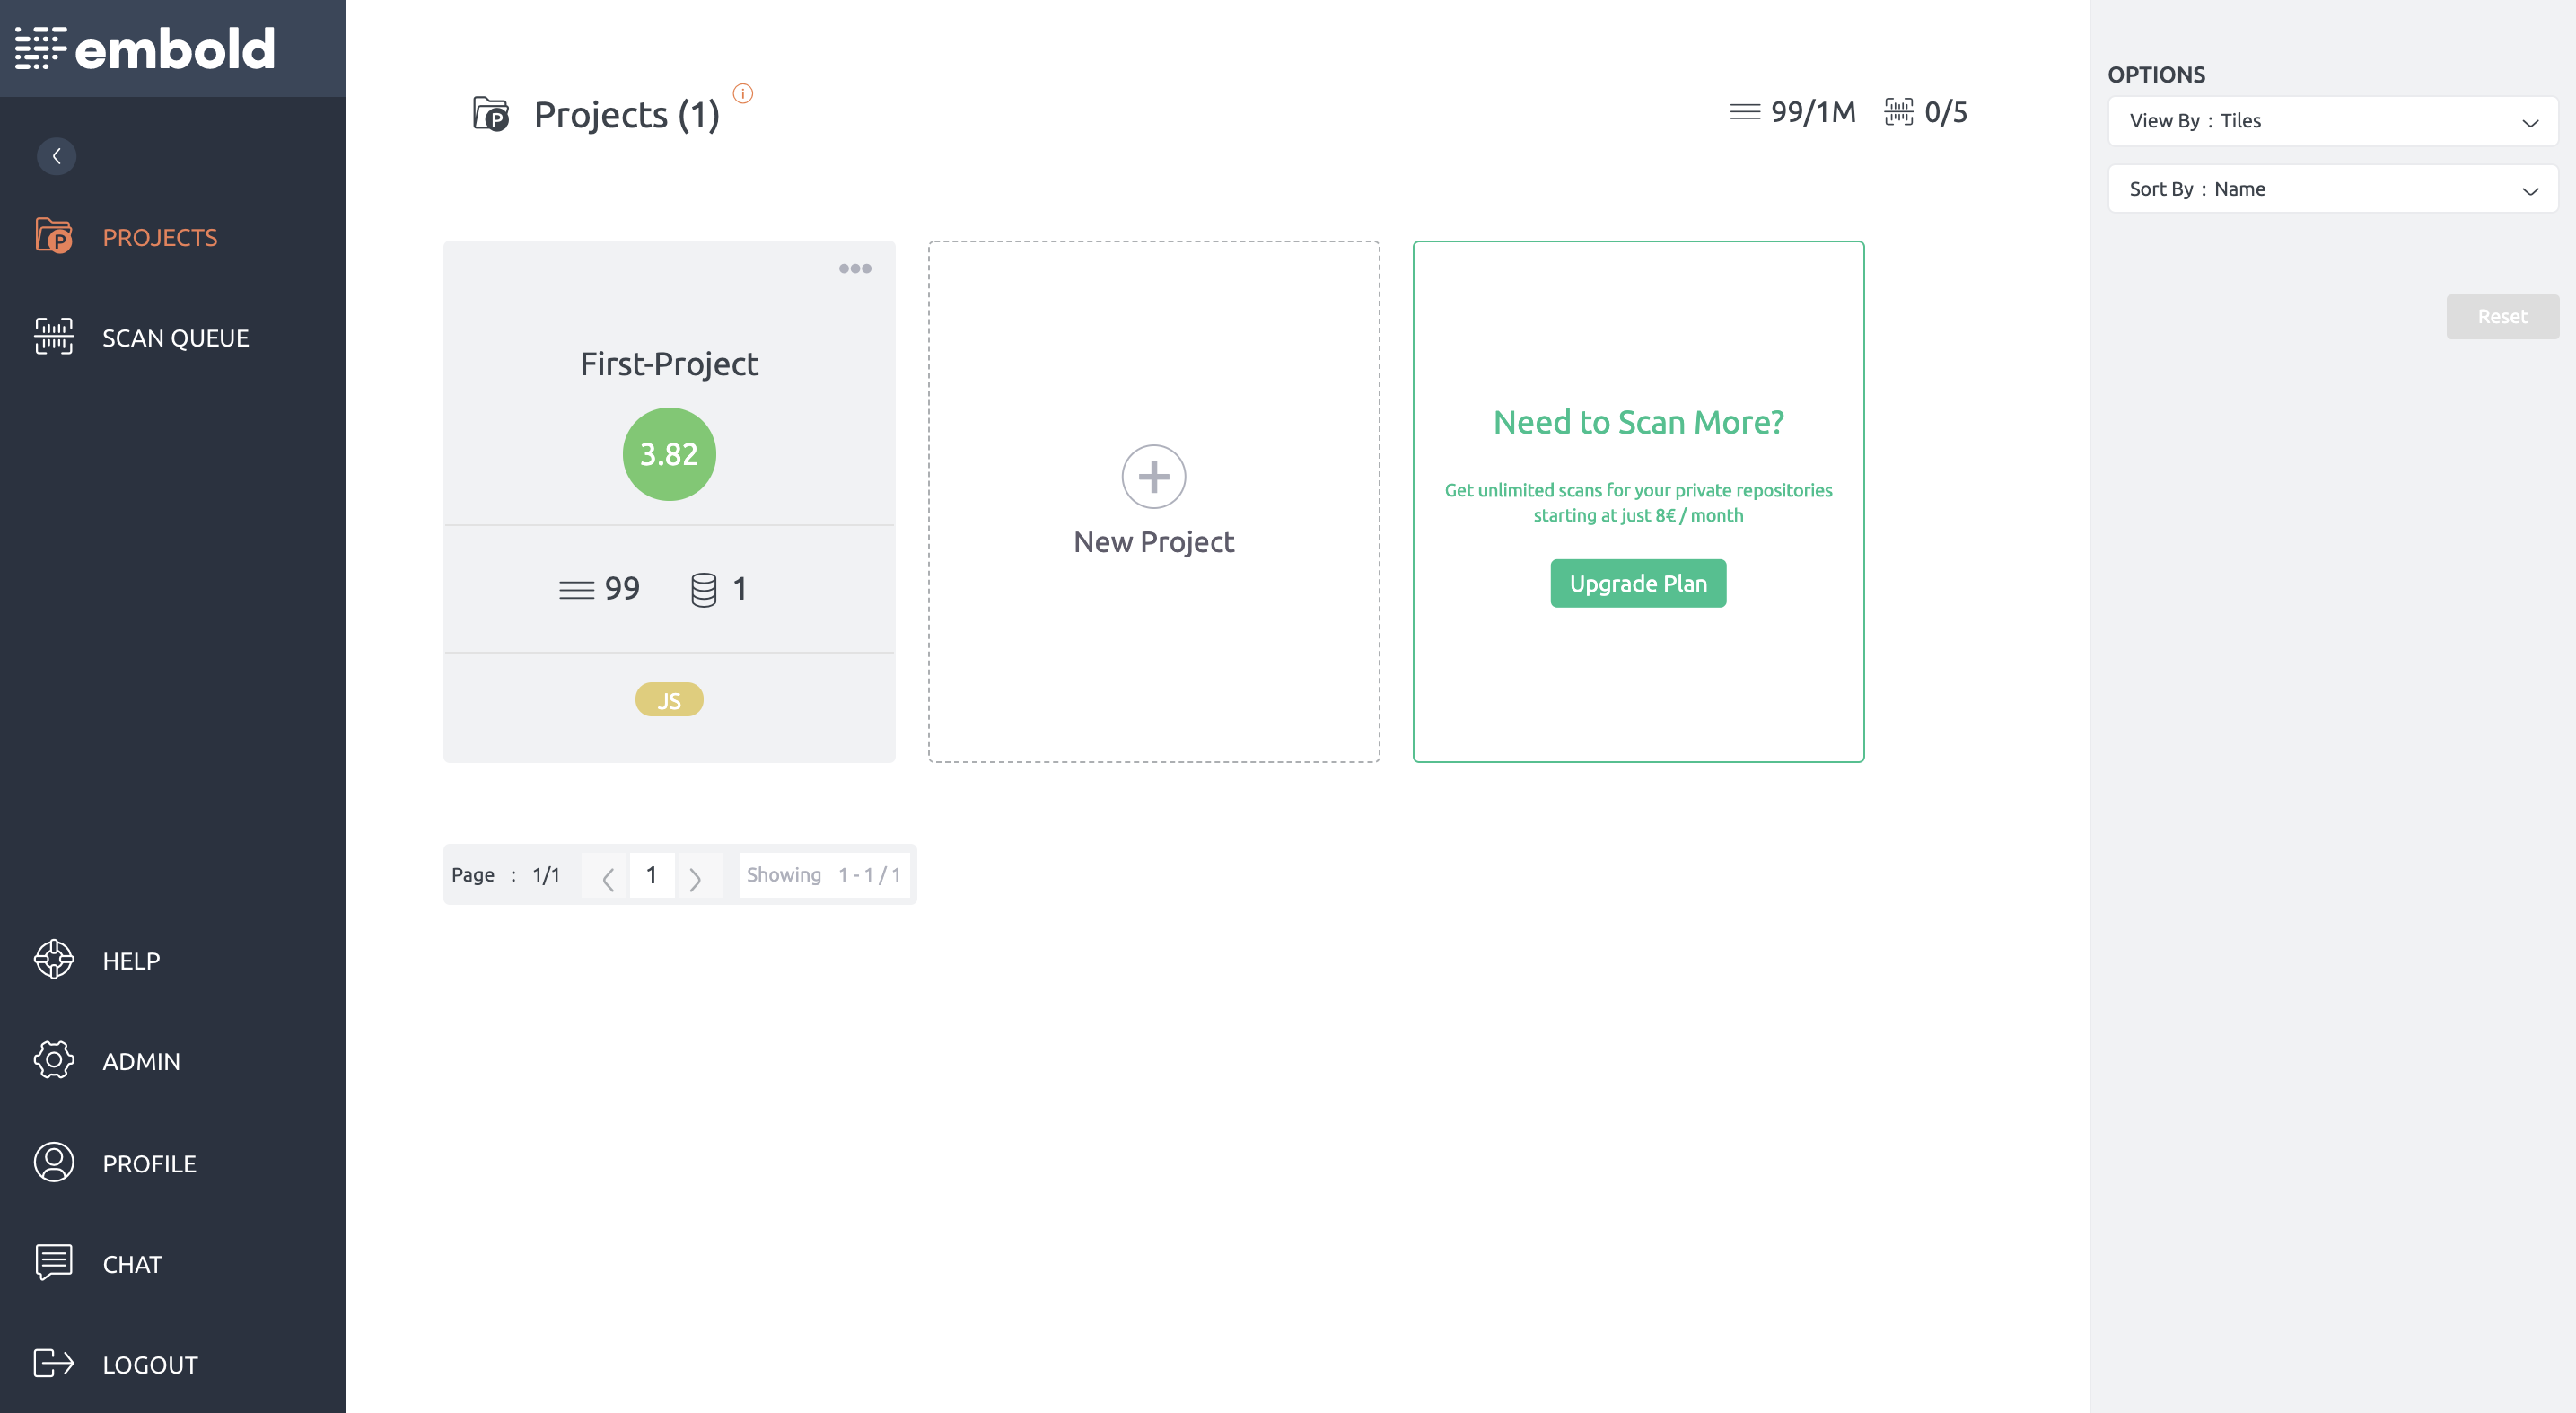
\includegraphics[width=6.5in, height=2.8in]{task-model.png}
\caption{Task Model ~\cite{emboldio}}
\label{fig:Task}
\end{center}
\end{figure}


\section{Scenarios}
The Embold is available as Open Source, Cloud and On Premise Self Hosted Environment. Various Pricing Plans are also available keeping in mind the need of the user. If somebody wants to use for once or just a few repositories it is free up-to 5 repositories but  all the repositories should be open source. \par
\begin{figure}[htbp]
\begin{center}
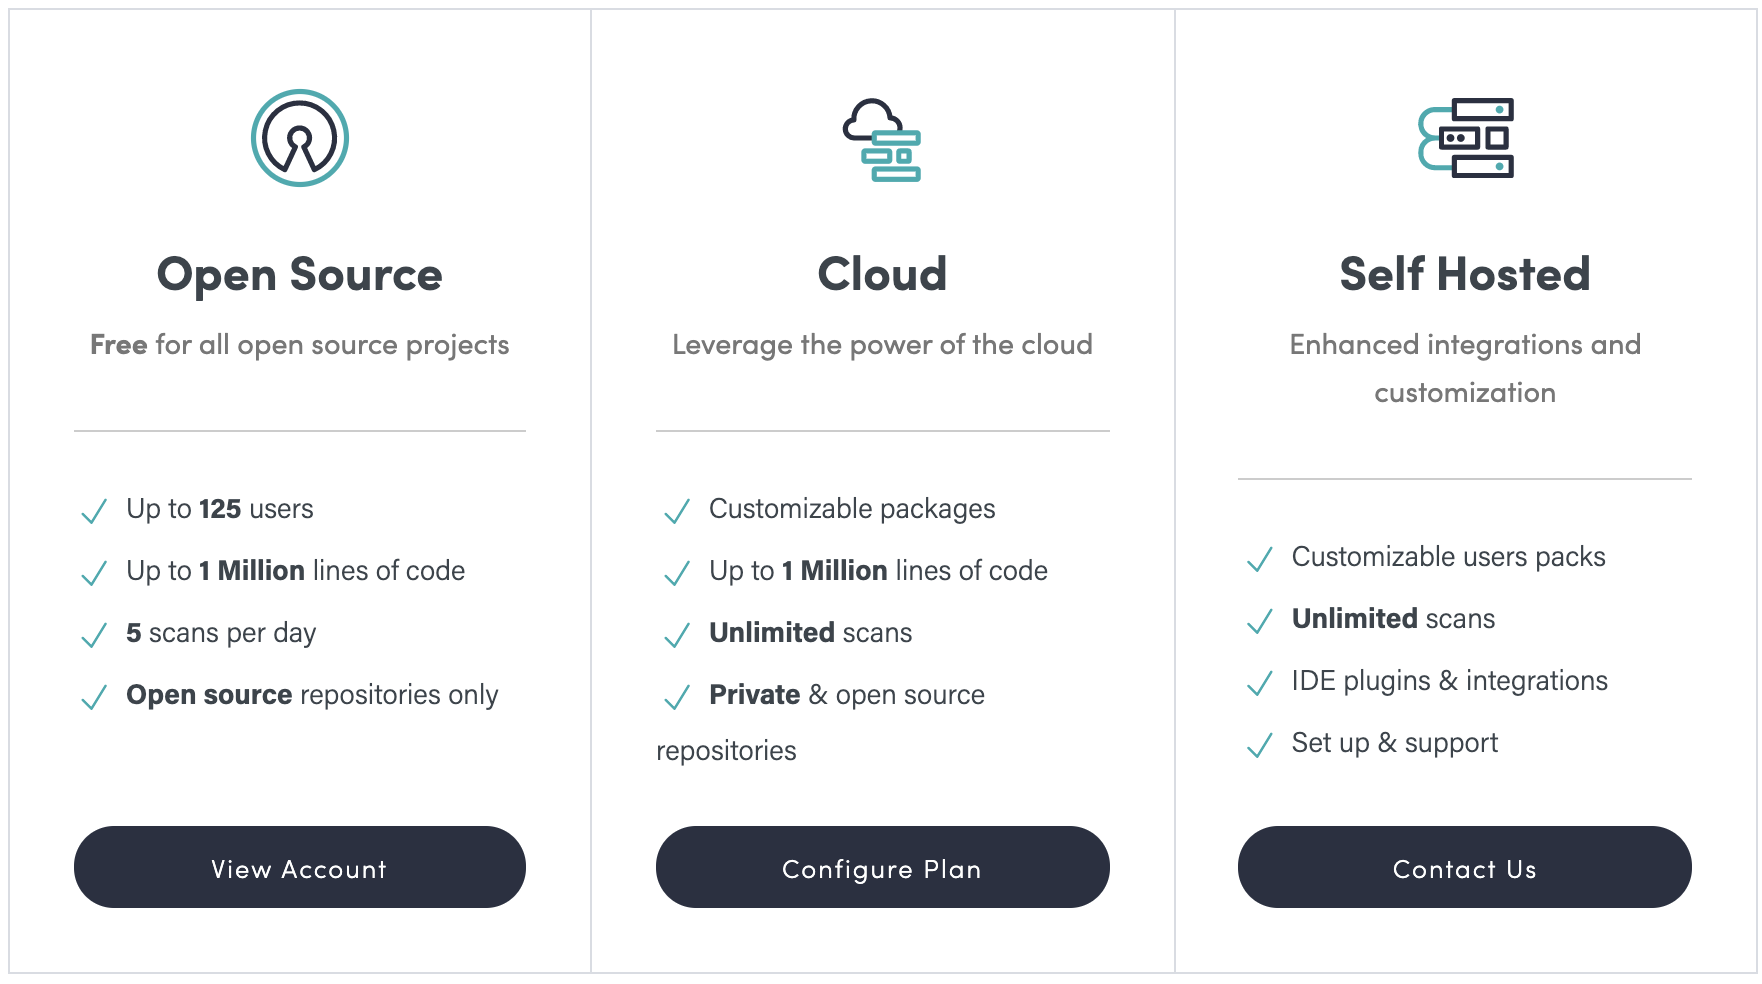
\includegraphics[width=6.5in, height=2.5in]{scenario.png}
\caption{Scenario ~\cite{emboldio}}
\label{fig:Scenario}
\end{center}
\end{figure}
\indent It has various price plans for the Start ups, Small Medium Enterprises and big Enterprises. As now world is moving towards the autonomous driving era, hence Automotive sector is using Embold eagerly, also few financial institutions are using Embold. The over view of the User Scenario is shown in Figure~\ref{fig:Scenario}.
\section{Persona}
I prepared a user persona of an Embold Developer as shown in the Figure~\ref{fig:User Persona}. As persona is just about an imaginary character, here Mr. Dane is the Software Engineer who has prepared the tool Embold. He has different and interesting programming skills as well as he has  comprehensive management and other soft skills. Hence he wants to develop a tradition to write the clean code so he very motivated and working to the Embold to new heights where all the user groups can perform their tasks very efficiently. Mr. Dane is also committed to   include more programming languages which can be analyzed using the Embold.
\begin{figure}[htbp]
\begin{center}
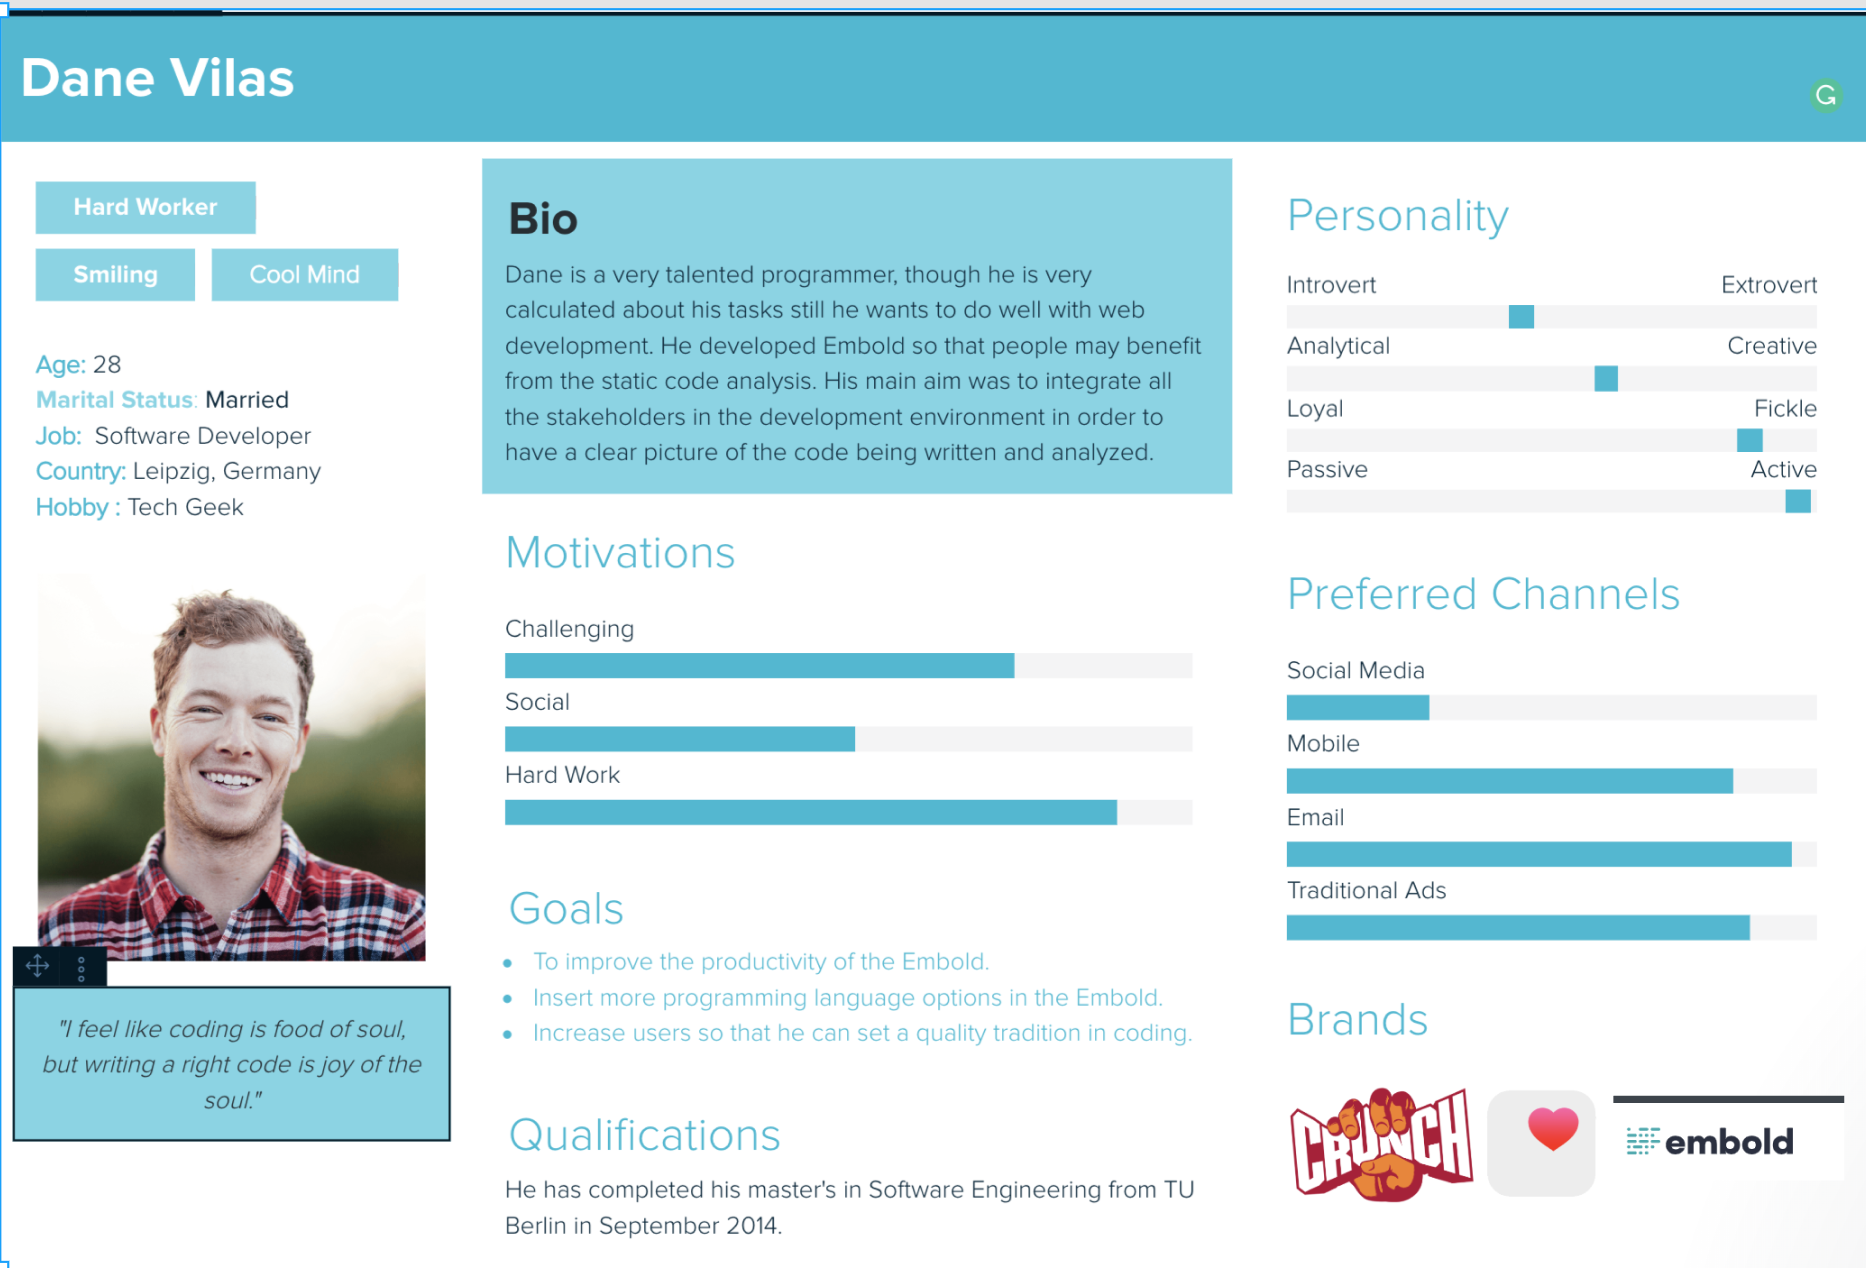
\includegraphics[width=6.5in, height=6in]{persona.png}
\caption{User Persona ~\cite{persona}}
\label{fig:User Persona}
\end{center}
\end{figure}


%chapter2
\chapter{User Requirements}
User requirements are actually the expectations of the the client. Either it's the solution of a specific problem inside a product or its completely a new product, requirements are highly important. Most of the projects fail due to bad or incomplete requirements. User requirements are the building block of any project and are saved in User Requirement Document (URD). Business Analysts are suppose to prepare the user requirements, they write, manage and keep track of the requirements. Modern day projects are all about the change and change is the most consistent thing which happens in the project. So Business Analysts also are responsible for the change management in the Project.
\section{User Needs}
As we know that the good user needs are those which are testable. If we talk about Embold and its context of use, every user whether he is from any of the user group he will expect the Embold to to work with various version control systems. As a code analyzer the Embold has the feature to pull the repositories from the various version control systems like GutHub, BitBucket GitLab etc. So mostly users are very happy with this as its one of the most important requirement which is fulfilled. The open source, cloud and on premise availability of Embold is also a requirement depending on different Users. Providing the information code  issues, design issues, quality metrics is adding the value to product and that is the main focus of the user requirement to make the product Minimum Viable Product (MVP). Following could be the prominent user needs for an Embold user:
\begin{itemize}
\item Availability of the Embold as On-premise, and Cloud product so that user can test the code on their ease.
\item Availability of the Embold according to the size of the Enterprise for an efficient use.
\item Availability of the Embold with various functions for different stake holders like Quality of code and Road blocks  which not only benefits the developers but also gives an insight view of the project duration, time line and risk which is helpful for the Project Managers. 
\item Explanation about the Code Issues to keep the code clean.
\item Indication of KPIs such as reusability and maintainability etc. 
\item Information about the code Duplication. 
\item To have overview about various snapshots in version control system. 
\end{itemize}
\section{User Story}
Syntax of the User Story is; \par
\emph{As a ``type of user", I want  ``some goal ", so that ``some reason ".} ~\cite{story}\par
User story is about a specific type of user who want to perform a specific task in order to achieve a specific milestone. In agile methodology the concept of `CCC' is very important to understand what the user story is and how it works. CCC is for Card, Conversation and Confirmation. In Scrum methodology during the SDLC, teams works on various features of a product and depending on the nature of the feature complexity teams normally have a sprint of 1 or 2 weeks to prepare the feature. Requirements are moved to sprint backlog from the product backlog in order to start a sprint. Teams then select the features to be developed from the sprint backlog on the base of priority. While user story is the high level final description of the requirement which  developer is working on. In context of `CCC' user story is;
\begin{itemize}
\item\emph{Card:} A complete and pinpoint description of a component or feature. 
\item\emph{Conversation:} Teams discuss in order to explore more the functionality and make the component or feature a reality.
\item\emph{Confirmation:} Conducting the tests in order to confirm the functionality of the feature and reaching the stage `Done'.
\end{itemize}\par
User stories are short and accurate, normally do not have info how the feature will be developed. It is sometimes not shared with the client, but it must be short and should be written as by the users perspective. Each and every stage is very important in the user story whether is description of the functionality, conversation about the functionality or the unit testing of the component. ~\cite{Agile}\par
As Embold is a code analyzer it helps to confirm the user story and achieve the `Done' stage in any sprint.
\subsection{User Story in Case of Embold}
Someone who is either developer or manager, he will opt for the Embold when he wants to have the continuous testing and insight view about his project. Startups, SMEs and Big Entertprises use the code analyzer. \par Embold is used when a code review is required e.g an enterprise like SAP is developing a solution, they will probably use the Embold to check the quality of code,  the time required to finish that project, if they need to amend the design they need the static code analyzer like Embold. It will eventually give them all the info they want.\par
   %here I have to start again.
\section{User Requirement}
User Requirements in context of Embold user could be very simple to understand. To create a project that pulls the repository from the version control is the first thing which every user group would expect as shown in Figure~\ref{fig:Requirement}.\par
\begin{figure}[htbp]
\begin{center}
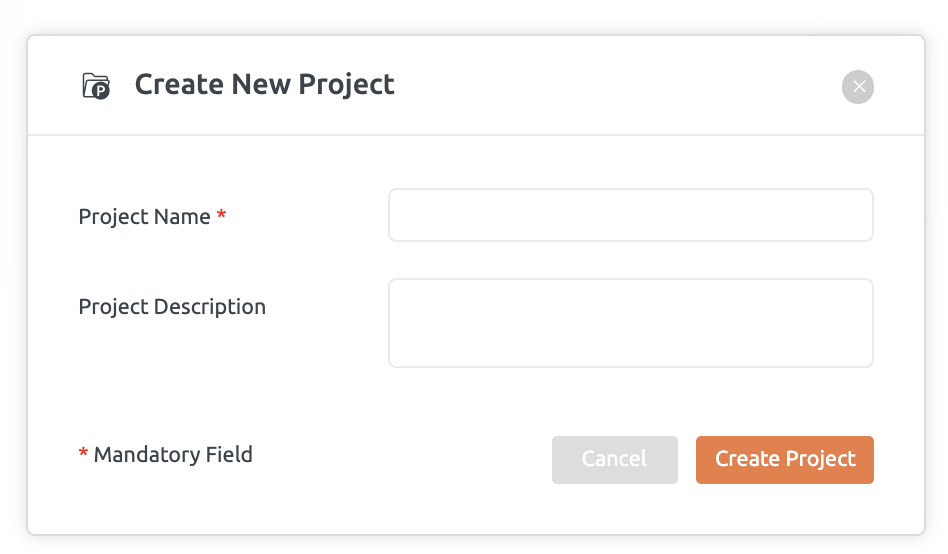
\includegraphics[width=4.5in, height=1.8in]{requirement.png}
\caption{User Requirement}
\label{fig:Requirement}
\end{center}
\end{figure}
The Embold Users have few more requirements about the code analysis, they would expect Embold to show them the result about the code issues, quality metrics, duplication, design and hotspots as well. These are pretty much functional requirements which Embold is fulfilling, as shown in Figure~\ref{fig:Requirement1}. \par
\begin{figure}[htbp]
\begin{center}
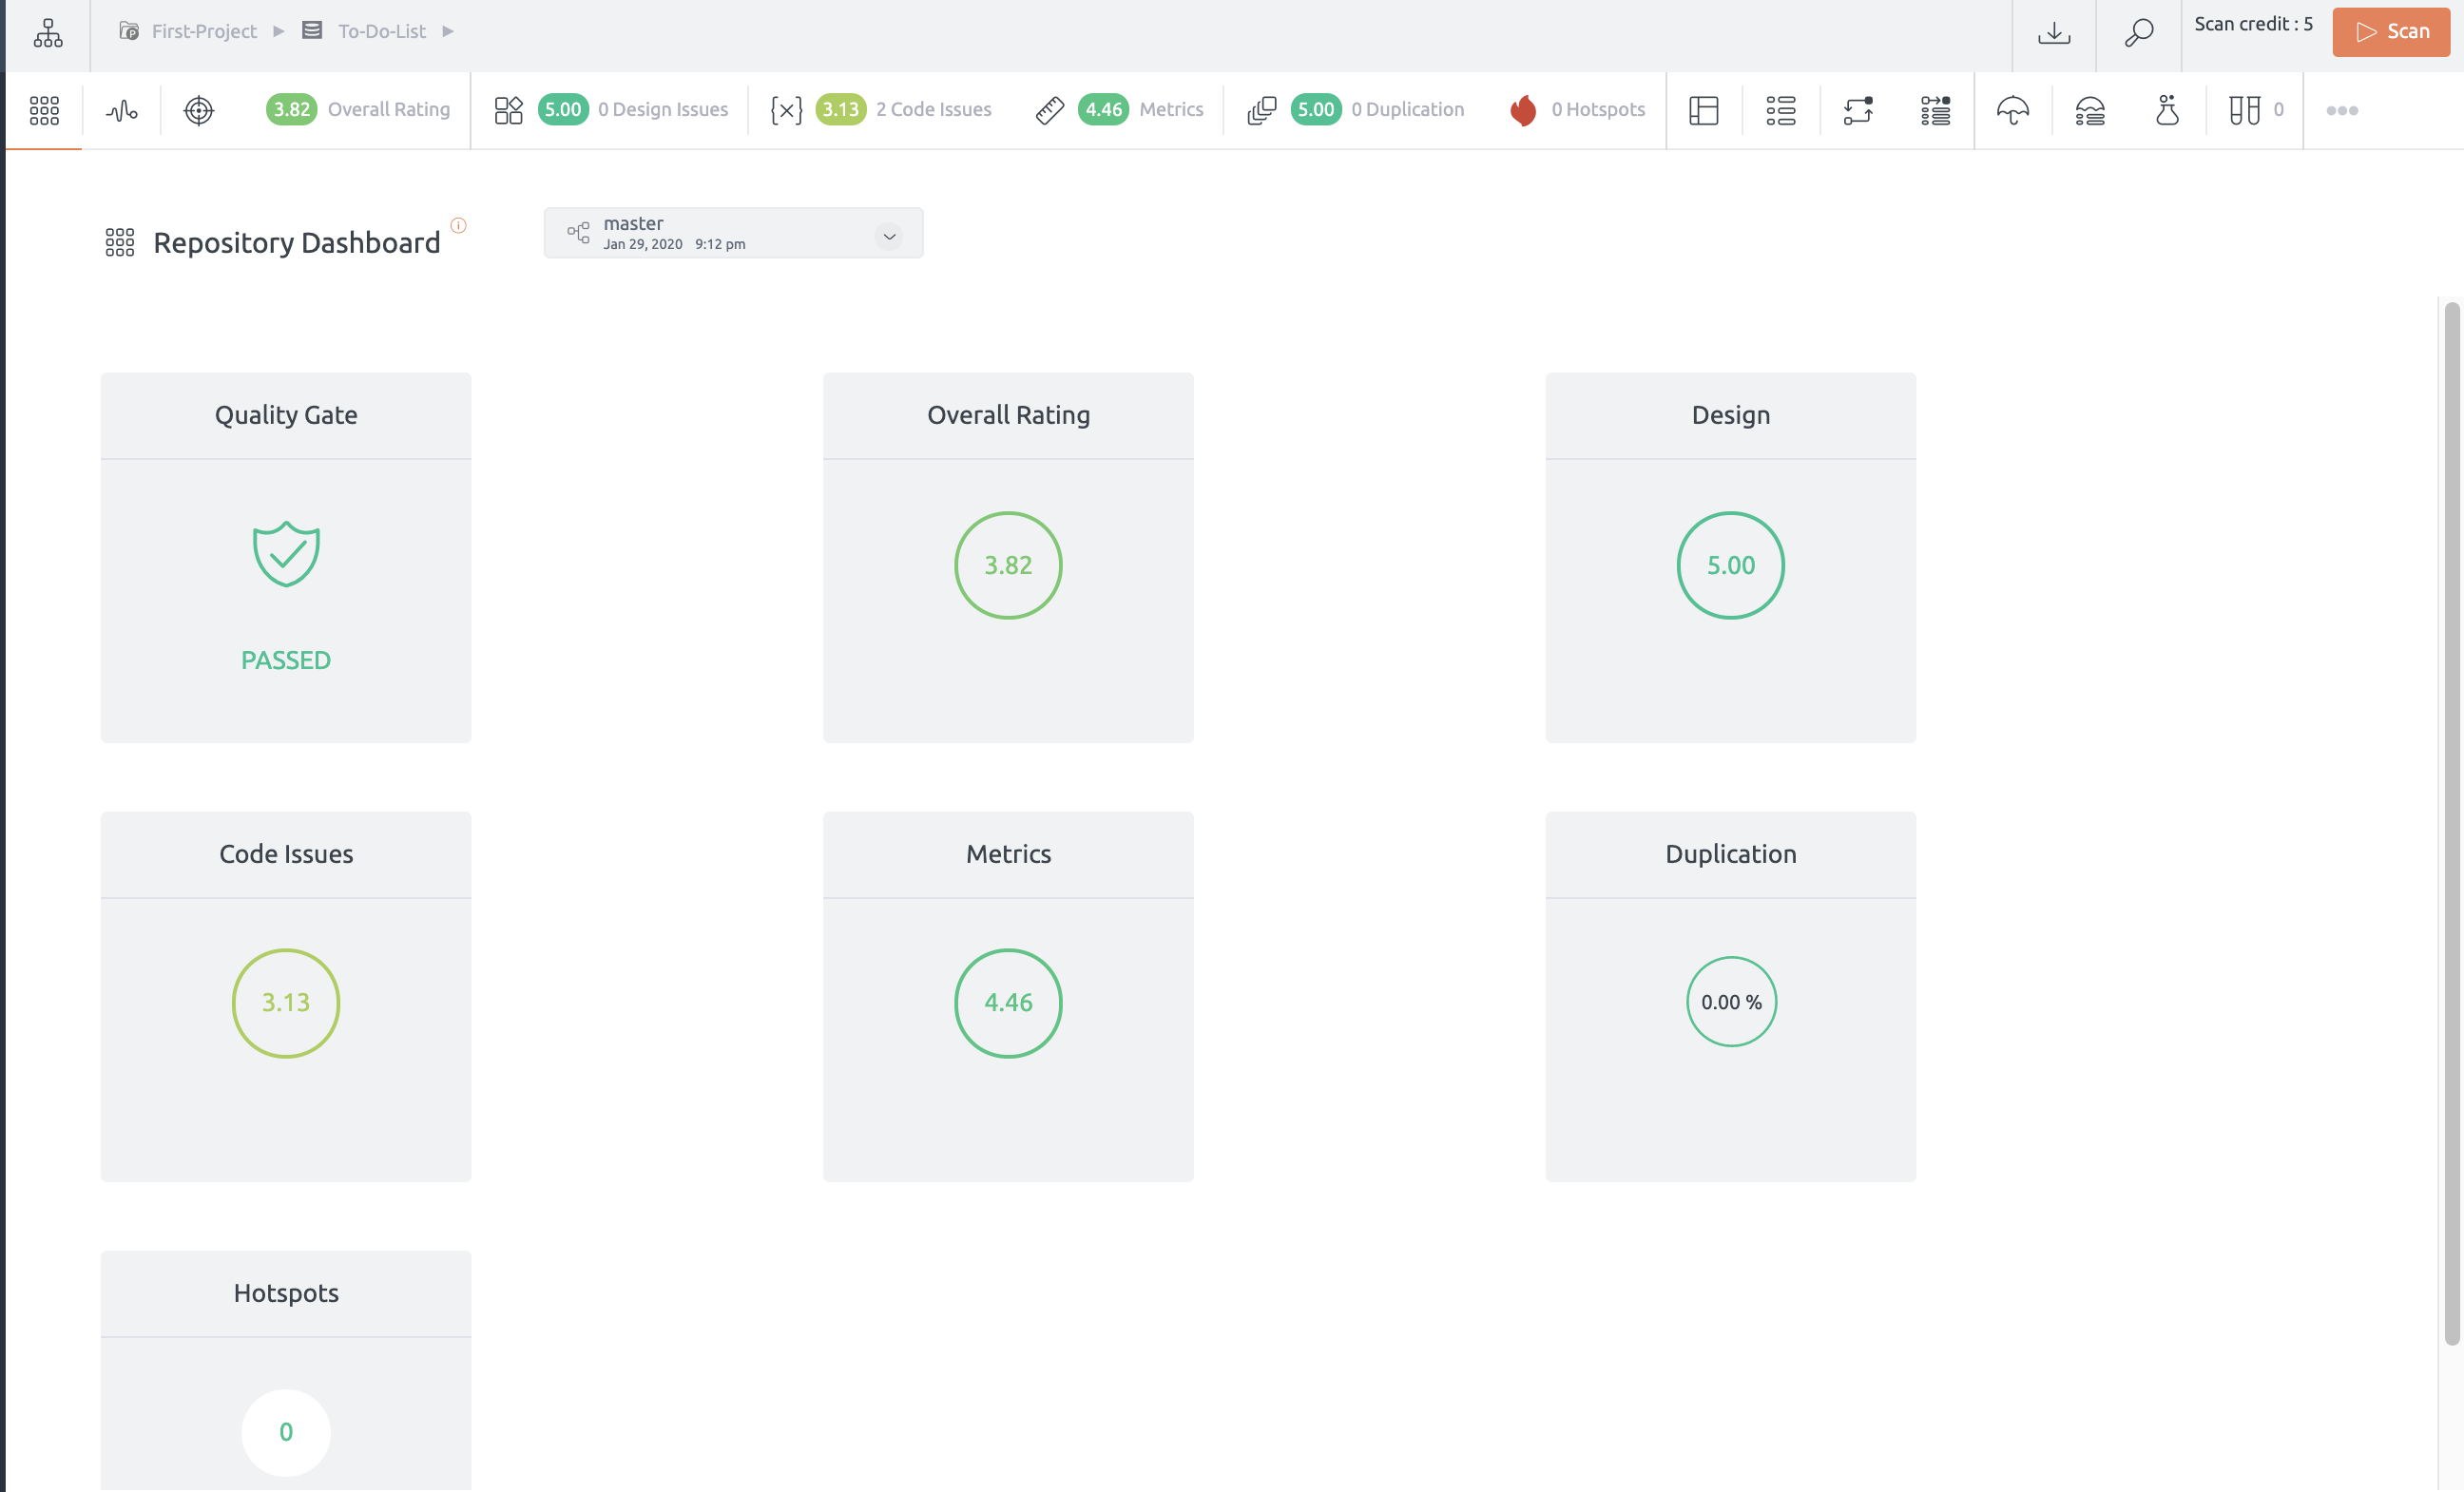
\includegraphics[width=6.5 in, height=3in]{requirement1.png}
\caption{User Requirement as an Output}
\label{fig:Requirement1}
\end{center}
\end{figure}
If we further delve into the output which we have in Figure~\ref{fig:Requirement1} we can notice that there are more detailed functionalities which are the important requirements of the user. More detail about code issues, metrics, hotspot etc as shown in Figure~\ref{fig:Requirement2}.\par
\begin{figure}[htbp]
\begin{center}
\includegraphics[width=6.5 in, height=3in]{requirement2.png}
\caption{User Requirement as Output in Detail}
\label{fig:Requirement2}
\end{center}
\end{figure}
Apart from all these the response time which the Embold takes to scan any project is also quite important. Embold also gives users to online help, info about price plans and also an ease to manage their profile using the options available in the profile as shown in Figure~\ref{fig:Requirement3}. All these are non-functional requirement which have a big impact on the product. 
\begin{figure}[htbp]
\begin{center}
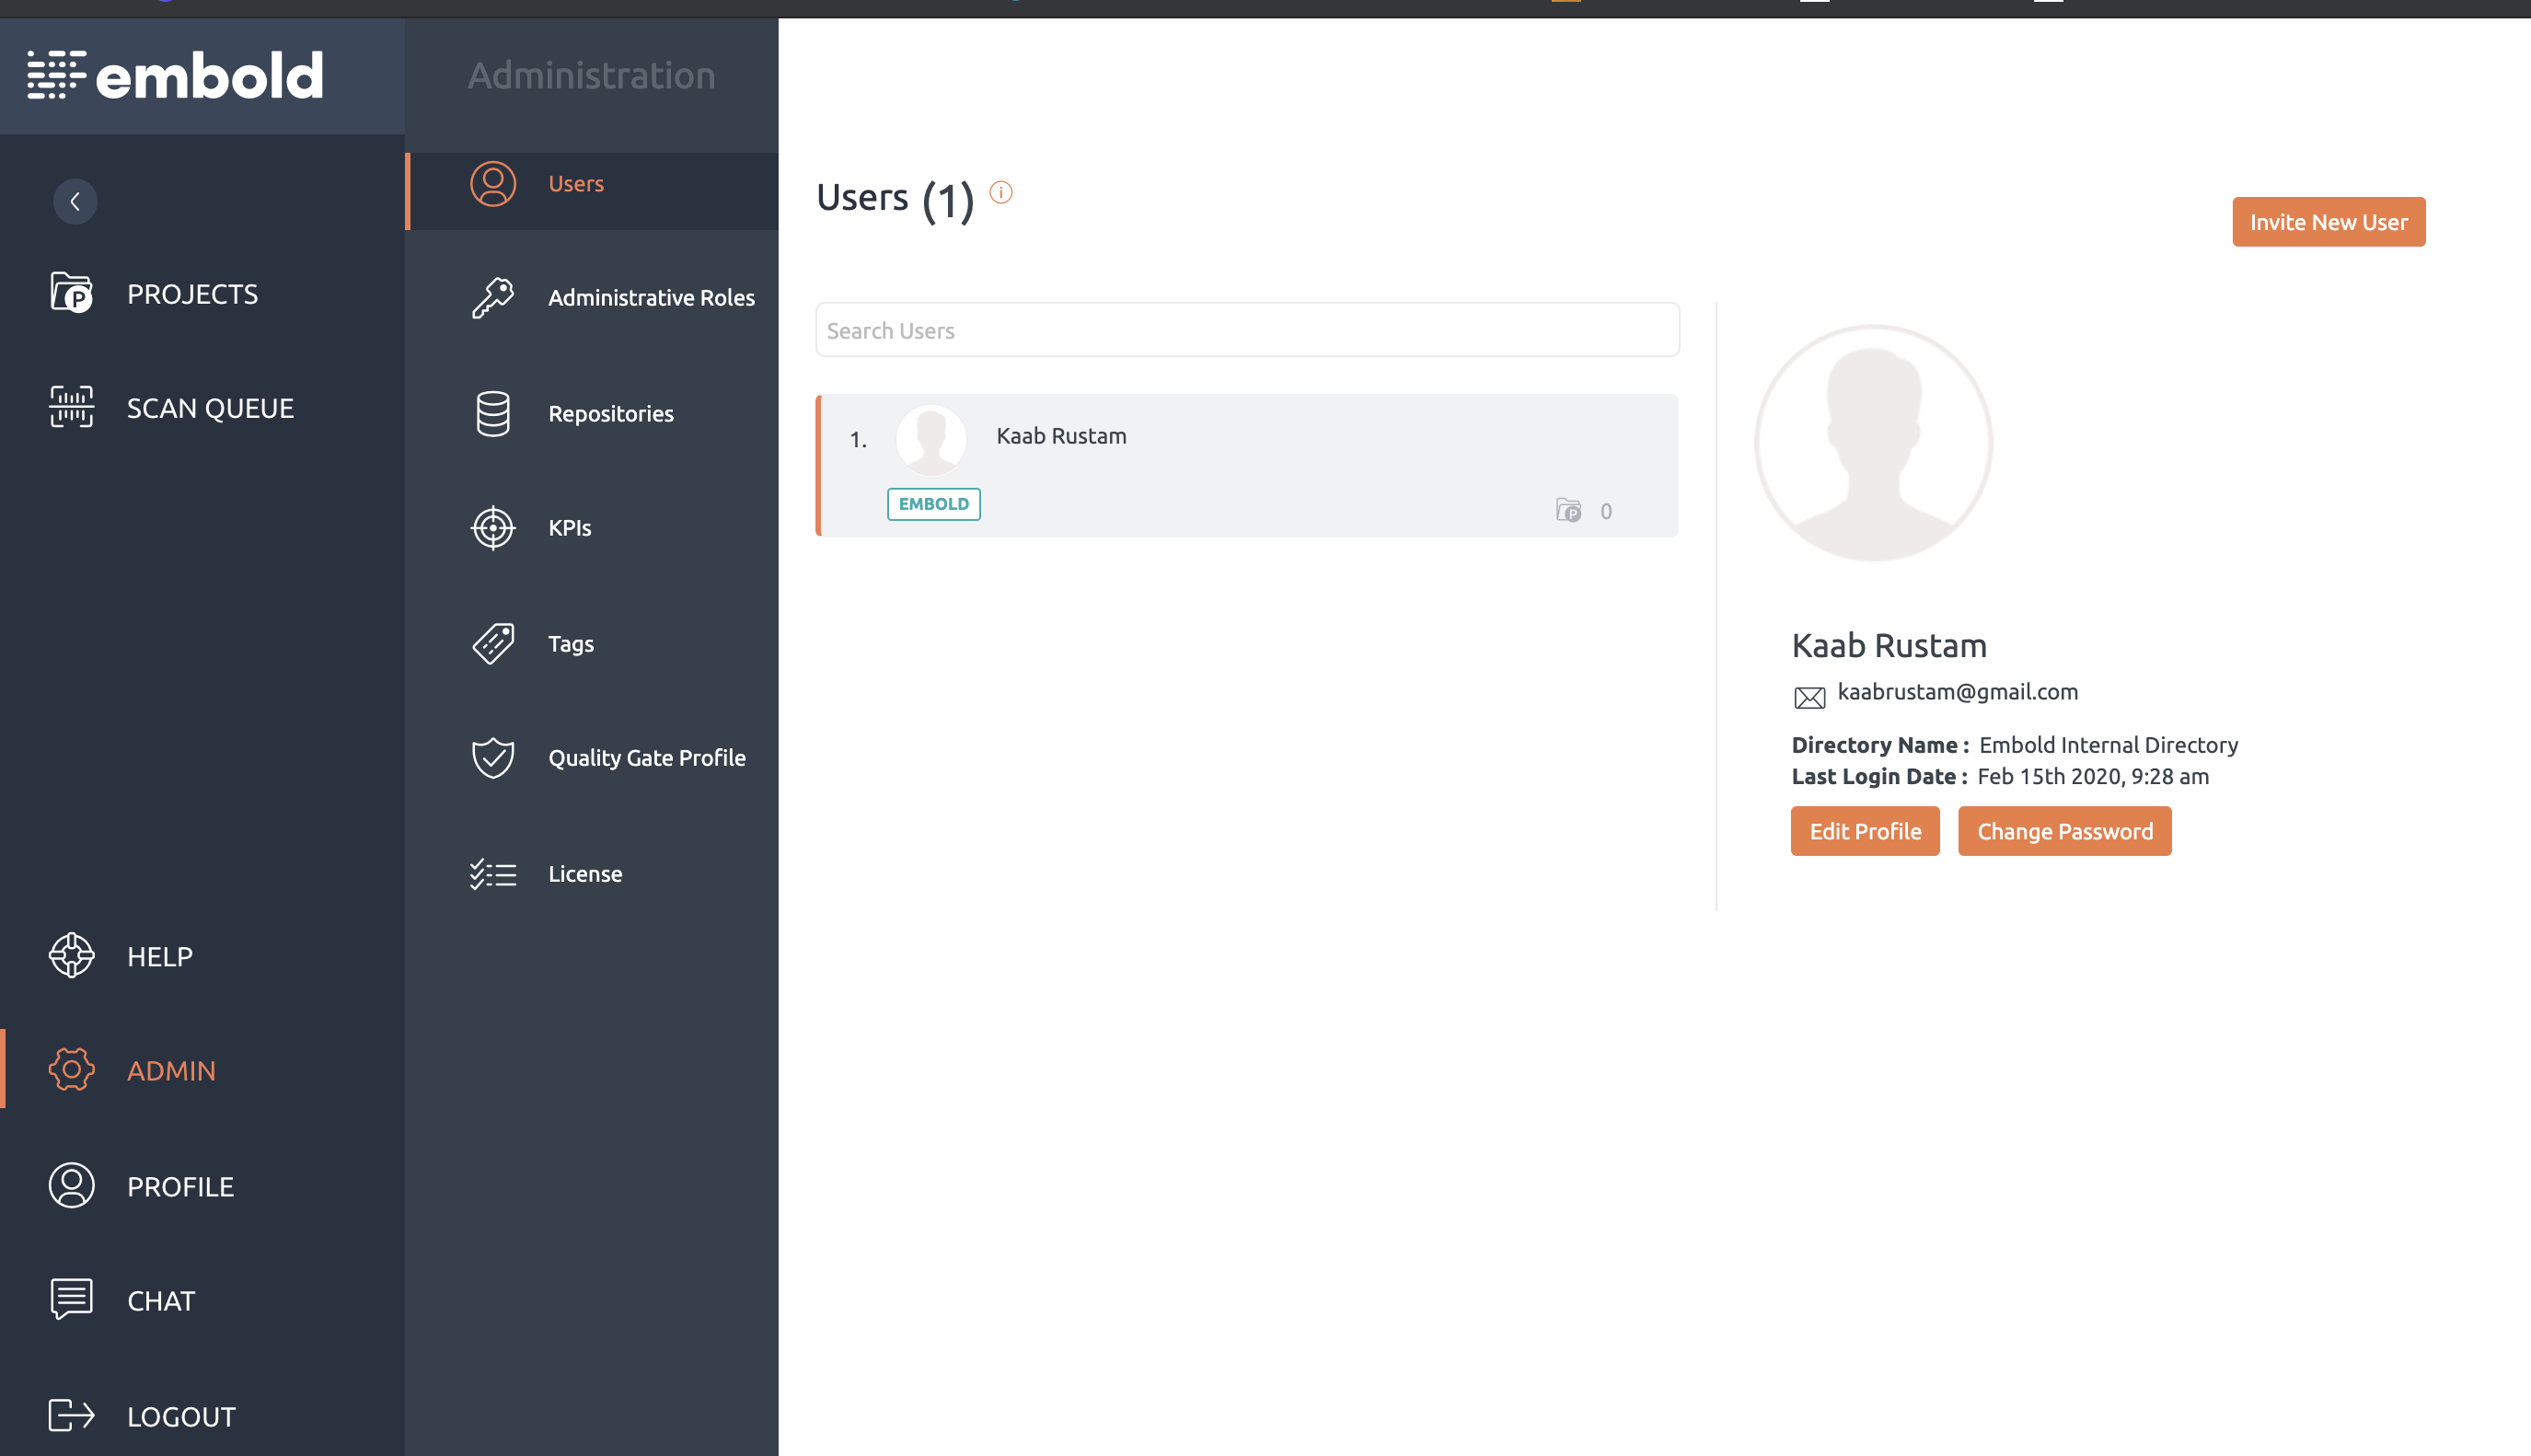
\includegraphics[width=6.5 in, height=2.6in]{Requirement3.png}
\caption{Non-functional Requirement example} 
\label{fig:Requirement3}
\end{center}
\end{figure}
\subsection{User Requirements Template}
We can illustrate the User Requirements as shown in Table \ref{tab:Requirement}
\begin{table}[h]

\begin{center}
%table starts here
\begin{tabular}{|p{6cm}|p{9cm}|}
\hline
\textbf{Requirement} & \textbf{Description} \\

\hline
Integration with Version Control & Embold SHALL Integrate with the any version Control. \\
\hline
Code Issues & Embold MUST  provide Information about the issues inside the code and code complexity. \\
\hline
Duplication & Embold MUST Indicate of Code Duplication in order to make the code clean and compact. \\
\hline
Adding Peers &Embold MAY Invite the other team members and control what the y can do with the Project. \\
\hline
Deployment History & Embold SHALL  review all the push and pull history in order to see code completely. \\
\hline
Dependencies & Emold MUST go through all the dependencies to analyze and regulate the code. \\
\hline
Support & Embold MUST provide the support for its users, while Embold MAY provide online support.\\
\hline
\end{tabular}
%table ends here
\end{center}
\caption{User Requirements Template}
\label{tab:Requirement}

\end{table}



%chapter3
\chapter{Product Design}
\section{Information Architecture}
If we talk about User Centred Design and modern day solutions, one of the most important thing is ``Information Architecture". It is the feature which clearly indicates the quality of the product, UCD is so crucial that extremely complex algorithms are designed to focus on the user needs and to focus on type of the user. It may take several iterations to create a presentable information architecture. In order to match high degree of usability the focus is very deep on the information architecture. It is the feature that helps navigate the complete product without any serious effort or without consuming much time. A good information architecture has property that users can quickly understand what the navigation says. Its very crucial to use easy and meaningful navigation in order to have quality information architecture and pleaseant usability experience. ~\cite{informationIA}\par
Embold has also an easy to explore information architecture, there is relevant information about various components, features and their functionalities.  If    we have a look on general navigation bar of Embold website and Embold tool, it has quite reasonable navigation bar. Website has the horizontal navigation bar as shown in Figure ~\ref{fig:horizontal}, and it contains a very detailed information about the tool, price plans, enterprise categories and much more. A user can easily understand as it's a good usability experience, user centred design and quality standards are kept into the mind while designing.\par
\begin{figure}[htbp]
\begin{center}
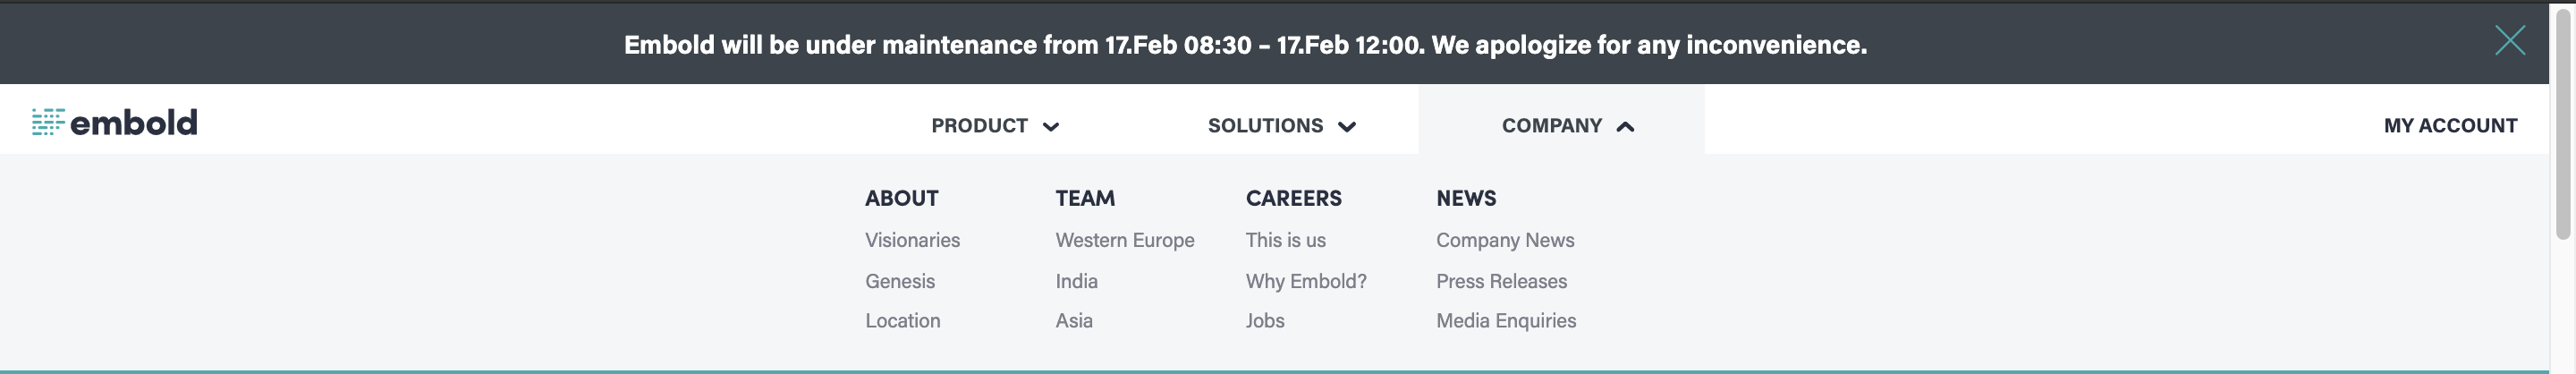
\includegraphics[width=6.5 in, height=1.7in]{Horizontal.png}
\caption{Horizontal Website Navigation}
\label{fig:horizontal}
\end{center}
\end{figure}

\indent Now if we look into dashboard navigation or navigation of the Embold Tool as shown in the Figure ~\ref{fig:vertical}.  It looks acceptable. As still there is a room of the improvement. There could be detail information about the projects and other activities. But overall the information architecture is simple, easy to understand, it is hierarchal, logical and tag based. \par
If we talk about in depth Information Architecture is not actually UX Design, but a good Information Architecture leads a user for better UX Design and usability experience. Information architecture is based on the nature of the website and the content of the website. It truly depends on the product, the design team has to change the information architecture as per user needs considering a lot of things. Famous Information Architects Rosenfeld and Peter Morville mentioned in their book ``Information Architecture for the World Wide Web" that Information Architecture has four main components i.e 
\begin{itemize}
\item\emph{Organization Systems:}The approach used to categorize, classify and structure the available content .
\item\emph{Labelling Systems:} The approach of presenting the information which we have. 
\item\emph{Navigation Systems:}  The approach to move through the information, how to use identifiers in order to reach to a specific stage or to get a specific data.
\item\emph{Searching Systems:} The approach which enable users to search for their desired information. 
\end{itemize} 
If we need to understand and develop the successful Information Architecture, it is necessary to understand the user, their context of use and the content available. Because at the end we have to cluster all the data depending on the user needs and the way he thinks or works. ~\cite{IA} \par
So it is same for the  Embold, a user will look for the type of the plan available for the Enterprises. Also if we move towards the further task related activity, a user has ease to select the repository from his version. Also a user gets the detailed information about his code analysis. So the information is classified in categories and presented in a significant manner.\par
If we talk about the navigation system of Embold, it carries a lot of information which sometimes is not very much required. It does not have highlighting effect which can help us to differentiate the various identifiers in the navigation. Also there is the room  for the improvement in the fonts.  The navigation bar also does not include the most required features about search etc. We can not differentiate which is the navigation bar and which on is the information bar as shown in ~\ref{fig:vertical}. \par
While good thing about the navigation bar is that it provides some good information about the tool and it also lands us to the new page if we want to log in to the code analyzer. It also uses information bar to update us about all the changes, updates or any news related to Embold which is quite comprehensive.
\begin{figure}[htbp]
\begin{center}
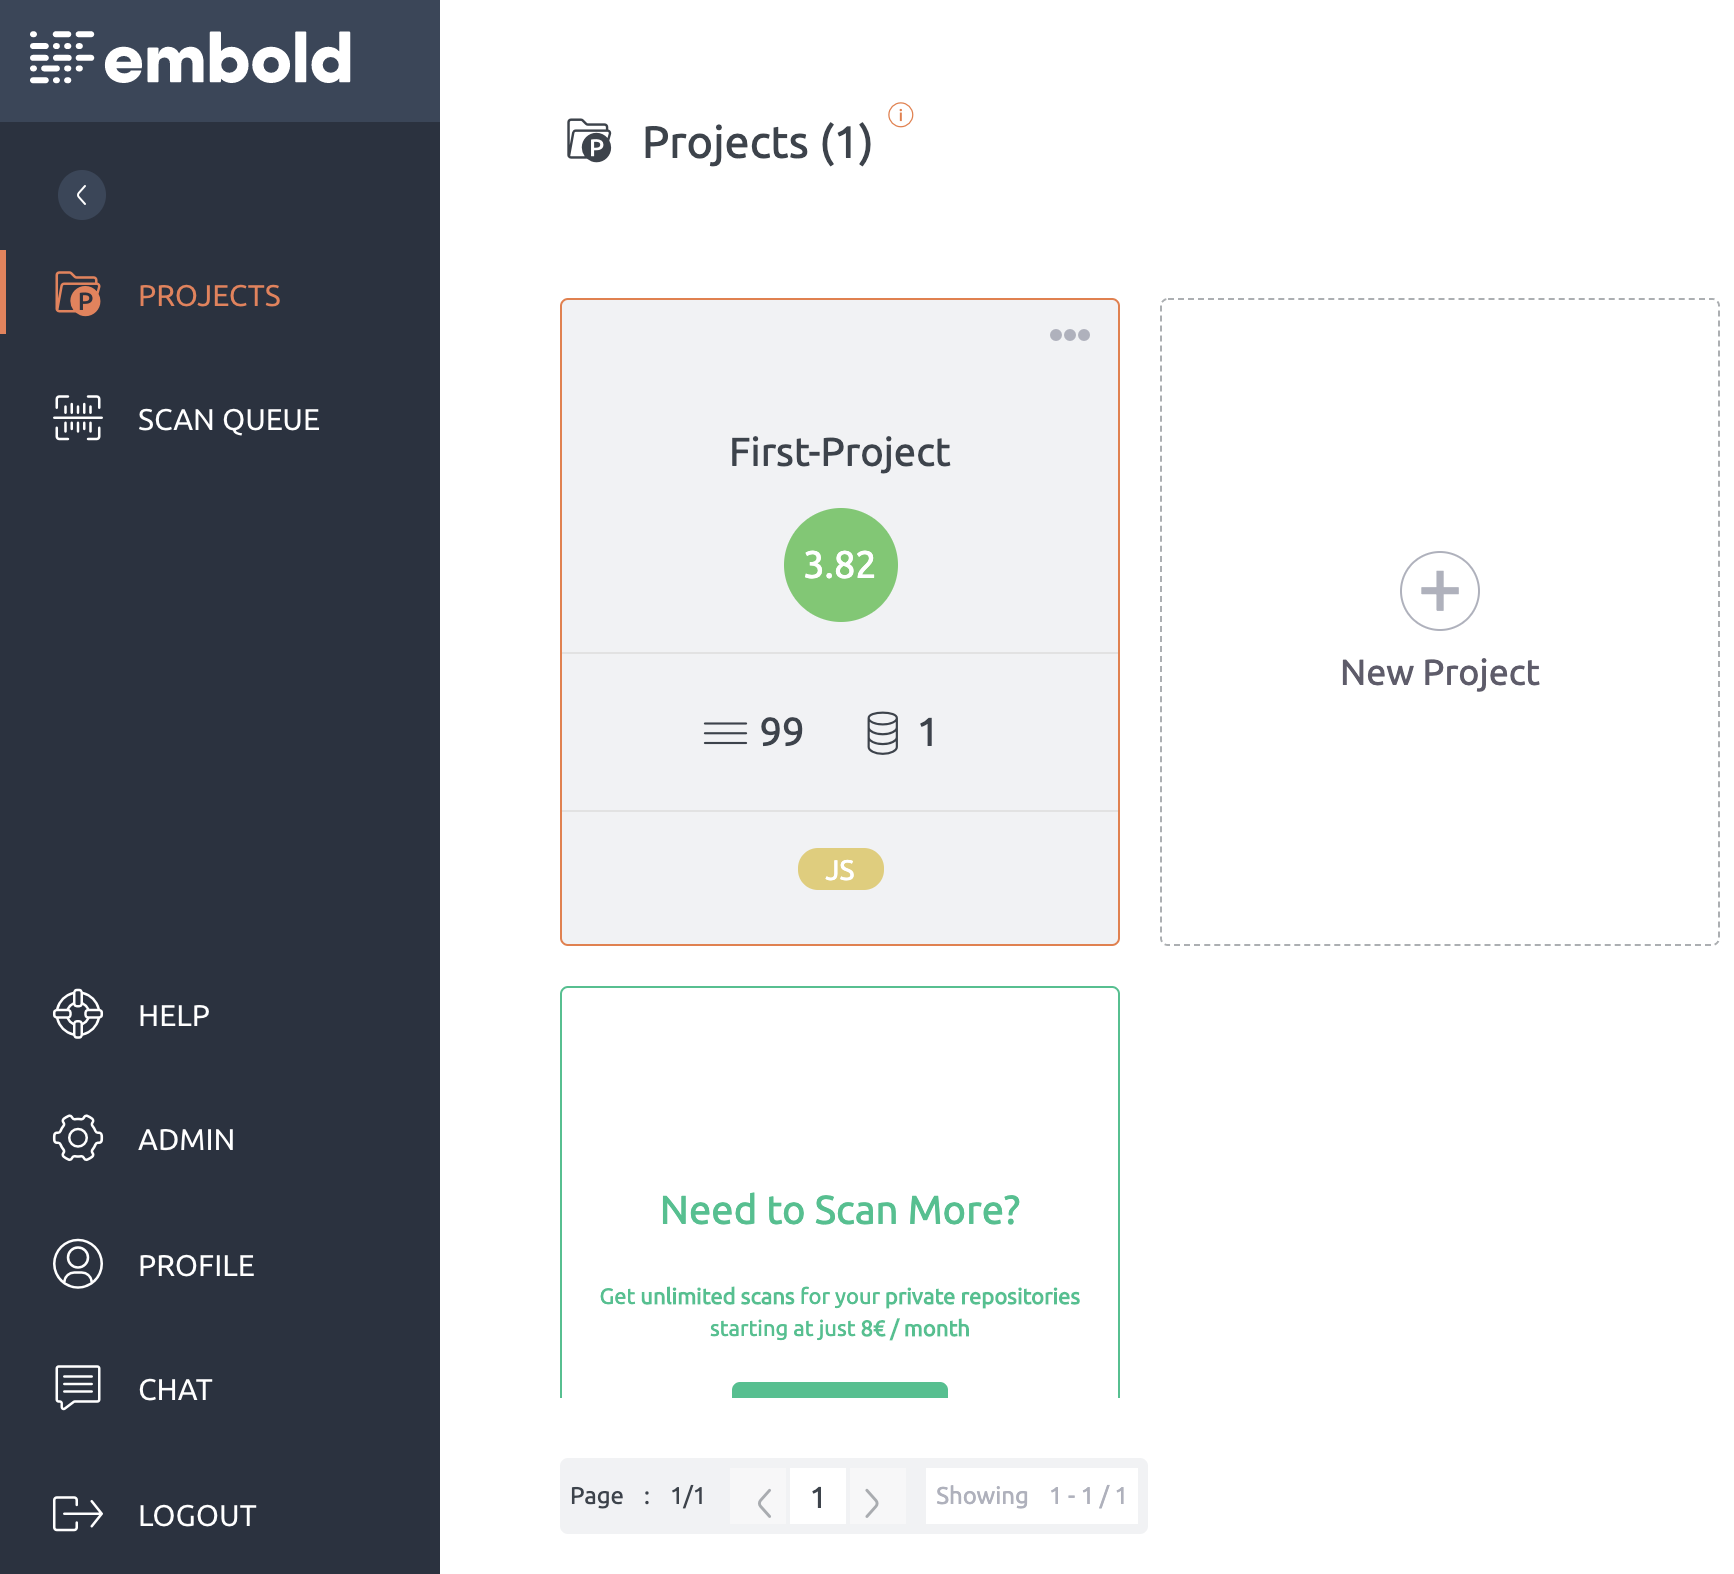
\includegraphics[width=6.5 in, height=3 in]{vertical.png}
\caption{Vertical Navigation Embold Analyzer}
\label{fig:vertical}
\end{center}
\end{figure}

\section{Style Guide - Comparison with ISO 9241-210}
Style Guide or UI style guide is somewhat the display of any solution and it is make or break feature of any product. Style Guide is an artifact of the design process and it  is created to bring together the Designer and Developer on the same page. It is very important for the successful production. Style guide is created by the UX designer. Before preparing a style guide it is important to classify the components of the style guide and have a clear idea what components merge to form a style guide. The figure ~\ref {fig:style} ~\cite{sguide} explains the overview of a style guide. It contains the information about the text style sizes used in the design. \par
\begin{figure}[htbp]
\begin{center}
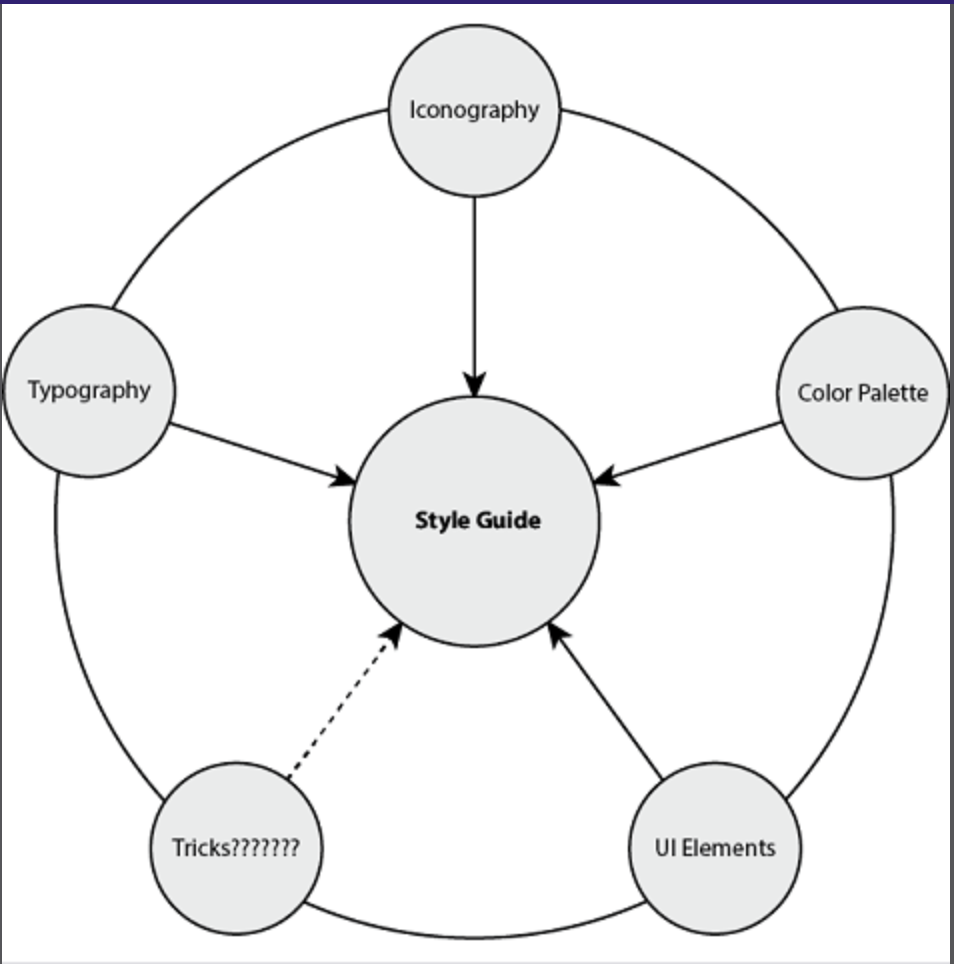
\includegraphics[width=4 in, height=3 in]{style.png}
\caption{Components of a Style Guide}
\label{fig:style}
\end{center}
\end{figure}
Style guide gives an accurate information about the colour codes, size of the buttons, form types, icons types and many other things which eventually help the developer in order to be on the same page with designer. All the User Interface (UI) designs have a style guide, UI is prepared considering the ISO standards about Human Centred Design and mainly User Centred Design.  SO it is very important to understand the ISO standards to produce a better product. Most of the times it's the UI  which pushes new users and explore the product more, in many cases users purchase the premium package just because of the UI design when they are at par with other products of the same UX Design.  So UI could be a tie breaker in few situations. \par
\subsection{ISO 9241-210}
If we talk about ISO Standard 9241:210, Human Centred Design for interactive systems; there are clear guidelines to develop useful and useable products. The scope of ISO 9241-210 is towards all of the design processes where both the hardware and software components of interaction systems can be used to enhance the Human System interaction.\par
The useful and usable products with better UX experience are developed by keeping in mind the user needs, user requirements and  HCD guidelines defined in ISO standards.
\begin{figure}[htbp]
\begin{center}
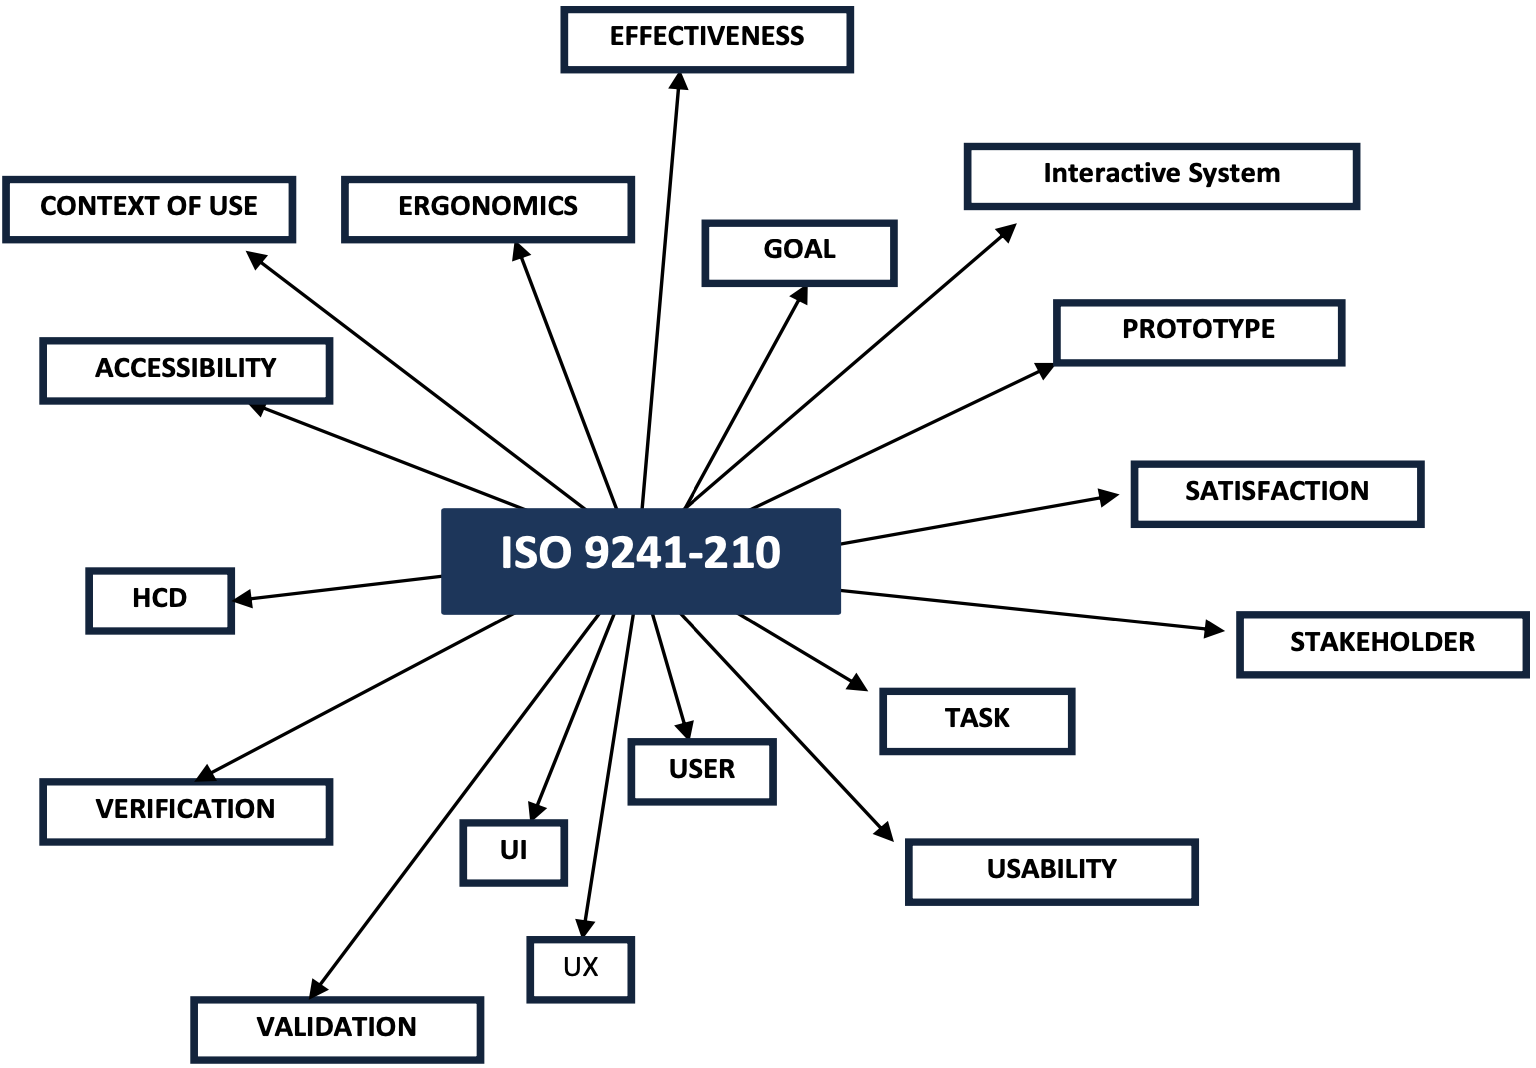
\includegraphics[width=4 in, height=3 in]{ISO.png}
\caption{ISO 9241-210 Features}
\label{fig:ISO}
\end{center}
\end{figure}
If we see the Figure ~\ref{fig:ISO} we can have a generic overview that what the ISO standard 9241-210 ~\cite{ISO} is about. It clearly defines a variety of aspects, whether it's about the user, user context, quality of the tool, functionality, tasks, goals and many other aspects. So before preparing any product is very helpful to consider all these aspects, which eventually help to yield in a very handy product. If I draw a comparison with Embold with these ISO standard, we can see a variety of aspects from Embold which will validate those features defined in ISO standards. For example a user is clearly defined, that someone with the Version Control Repository, and it validates before analyzing the code that the code which is being tested is coming from the version control. 
It comes up with specific goal, showing the various kind of results with a variety of descriptions available about the code quality, code issues, hot spots and duplication.  \par
A better UX is there as well, moving through the dash board is a seamless experience, a comprehensive logging in feature is available which moves quickly to the Embold dash board. 
If we talk about UI experience, it is not up-to the mark, as there is no clear difference between signifiers while hovering over them. The colour combination and schemes are not that which attract users. It is not as bad but still something which is below par to the standard. 
As Embold is a code analyzer, so it gives us option to add a variety of programming languages. It also comes up with many results which can help different user groups. It validates many aspects from ISO standard 9241-210, as it is being developed keeping in mind the needs of different users. Like a developer would love to see his progress, project managers would get a knowledge about the risks, potential delays and many other aspects, while the software architects get the actual design issues and all that with the progress of the real time project. \par
It is clearly as per ISO standards, that a user can the Embold according to his condition and requirement, a user can integrate it to any of the development environment. So overall user experience is up-to the mark which makes the Embold a useable and useful product. \par
While considering about user and their requirements, when a user will think about using Embold they will expect a good and readable out-look; they expect it to be easily access able. A user will expect the Embold to be compatible with the modern version control systems, they expect it to be available in various packages related to price and availability. They also expect it to provide information about bottlenecks, road blocks, quality of the software and also help about the estimation of finance and length of the project. \par
Now if we say that whether the Embold has meet up the use expectations, its not very difficult to answer as it has meet up the expectations as far as functionality and security is concerned. While there is room for improvement  in the design, display and outlook.  


%chapter4
\chapter{Evaluate the Design}
The design evaluation is something which is done to test the functionality of the products. It is kind of evaluation which makes sure that people can navigate through the website or application without any hurdle and the whole interface process is smooth. The process of `Heuristic Evaluation' and `User Testing' can be used to test the design of the website. The major difference between both the evaluations is that heuristic evaluation is done by usability experts while user testing is done be ordinary users. Thats why heuristic evaluation is referred as an expert review and is considered as more genuine and helpful. \par
The major enterprises which have enough resources normally make sure that the product is being reviewed by three usability experts. There are a number of criteria which can help testing the usability of the website. Once the guidelines are set for the evaluation each of the usability tester tests the website separately. Having multiple evaluators help to catch the diversity and have a holistic view of the design and improve the deficiencies and errors. While if we talk about someone who cannot afford the usability experts it is possible to conduct heuristic markup by own. But this is the process which is highly time consuming, one has to go through the whole design by their own and trying various combinations.\par
Now if we talk about user testing, it is always helpful to conduct the heuristic evaluation during the the development process e.g during mockup design. In combination with user testing heuristic  evaluation helps to make websites functional and easy to use. ~\cite{test}
\section{Test Cases} 
Usability tests are conducted to test three major factor i.e Ease of Use, User Friendliness \& Efficiency.  ~\cite{sixsteps}
There is a specific process which is adopted to conduct a usability test, there are a few steps which can be followed to conduct a test as shown in Figure ~\ref{fig:usability}.
Each and every step is important in this process and it is very important that the result of the test are incorporated properly. It is required to follow the steps and put good enough effort on each step, because it is going to discuss the fate of the product. 

\begin{figure}[htbp]
\begin{center}
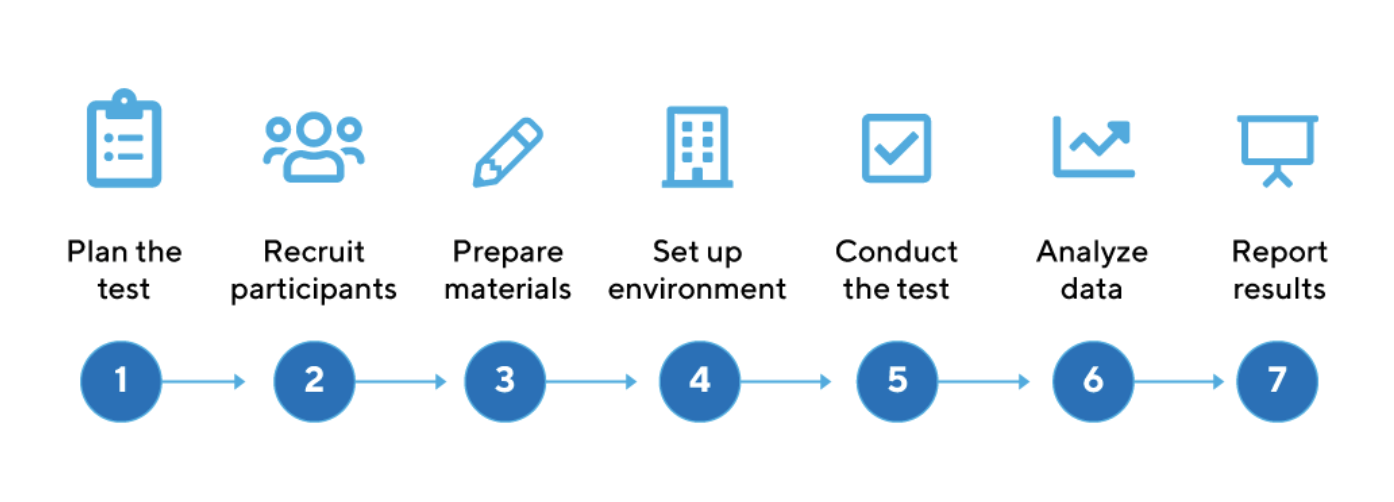
\includegraphics[width=6.5in, height=2.8in]{usability-testing.png}
\caption{Usability Test Steps}
\label{fig:usability}
\end{center}
\end{figure}
If we follow the templates and see the Embold as a test case, following are the take aways,

\begin{itemize}
\item Website is not efficient.
\item Problem in Navigation through the account and the Dash Board.
\item Hovering issues.
\end{itemize}

\section{Test tools \& Metrics}
Metrics are used to quantify the usability of any product. It is a standard which  is used to describe more than one attribute of any product. There are many secondary reasons to use the metrics i.e for a better communication with stakeholders, comparing the product with other same type of products. But the primary purpose is to yield a quality product which has considerably good user experience.
There are a number of ways we can use to test the UX design, we can use google analytics to have and educated guess and few other ways to test; number of users, their activities etc.  \par
We can utilize the concept of Behavioural and Attitudinal KPIs to measure the usability. Both these terminologies can be very briefly classified as: ~\cite{tools}
\begin{itemize}
\item Behavioural KPI (What it does)
\item Attitudinal KPI (What they say)
\end{itemize} 
Now going in detail of each of these KPIs;
\subsection{Behavioural KPI (What it does)}
It is a quite cheap way of collecting the KPIs and its kind of numerical KPI to evaluate the design. There are 4 major KPIs which fall under this category. \par
\textbf{\emph{Task Success Rate:}}\par
\indent If we talk in context of Embold, we can say its a measure of tasks completed successfully i.e, the logging in, trying to connect the Git Repository, successful scanning of the repository. 
Iff 10 people are given a task to do to test the tool, while 7 are able to do the task successfully then TSR could be calculated as :\[TSR= 7/10*100=70\%\]\par
\textbf{\emph{Time-on-task:}}\par
This KPI indicates the time spent to complete any specific task. Its actually average which is calculated considering the various tasks. Shorter the task, better the user experience. In case of the embold, I did spend much time on navigation and finding the indicators. So its user experience was not very great. \par
\textbf{\emph{Search Vs Navigation:}}\par
It is very handy if a user does not have to use SEARCH feature. So it is degree of usage of Navigation bar and Search bar. More the usage of search bar, weaker is the user experience. But in case of Embold, there is no Search Bar in the main web page, which is indication of poor user experience. Though the website has the search bar in the account inside but the UI is not of better quality as it is difficult to differentiate. \par

\textbf{\emph{User Error Rate:}}\par
The number of times any user makes the wrong entry, is considered as User Error Rate. It gives idea of how user friendly a website is.  The higher the rate of error, higher will be the usability problems. For example if a user tries to insert the date of birth in his name section, it should be an error and should be predefined, as name section should not include integers and so on. \par

\subsection{ Attitudinal KPI (What they say)}
It is about the feelings of the user, how the user feels and express their experience about the website. \par
\textbf{\emph{System Usability:}}\par
This section is kind of survey, which has 10 possible questions and 5 options to answer. It ranges from agree strongly to strongly disagree. It is not very difficult to conduct such surveys,,, because the questions are very much straight forward. I have used the survey questionnaire to determine this KPI for Embold as shown in Figure ~\ref{fig:SUS}.\par
\begin{figure}[htbp]
\begin{center}
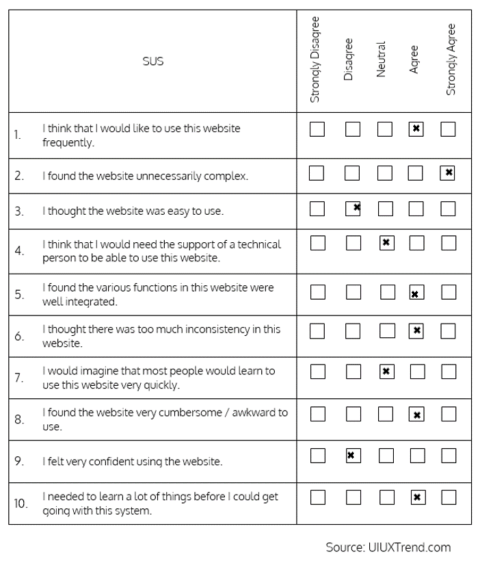
\includegraphics[width=4in, height=6in]{image.png}
\caption{System Usability Scale for Embold}
\label{fig:SUS}
\end{center}
\end{figure}
\textbf{\emph{Net Promoter Score:}}\par
It is about the referral of website, as it is just one liner question e.g ``How likely is it that you will recommend our website to the friends, colleagues etc". The answer ranges from 0-10 and categorized as:
\begin{itemize}
\item Detractors: 0 to 6
\item Passives 7 to 8
\item Promotors 9 to 10
\end{itemize}
from these 3 categories the `Passives' are ignored, and rest of the calculation goes like \[ (Number\ of\ Promoters - Number\ of\ Detractors) / (Number\ of \ Respondents) *100\]
\textbf{\emph{Customer Satisfaction:}}\par
This KPI asks about the satisfaction of the user during their experience using the website. It has normally score from 0 to 100 and divided in 5 stages i.e very dissatisfied, dissatisfied, neutral, satisfied, very satisfied. In this only the satisfied answers are considered and later percentage is taken out.  
\section{Usability Test Report}
What ever the design is, it is based on the result mentioned in Usability Test Reports. It is very important to incorporate the results mentioned in this report. There are few steps which are followed to write a comprehensive test report. Designers use this report step by step to enhance UI and UX design. The report is comprehensive and it contains the description about the problems in the design. There can be the workshops and highlight video in the comprehensive depending upon the nature of the product and its complexity. \par
Video can include the user in action and the hurdles they face in performing the tasks. While the workshop results can be part of the report. Also results are prioritized according to their level of intensity, also the graphical solutions could be the part of the report in order to help the designers how the users can be engaged. 

%chapter5
\chapter{Conclusion}
\section{Summary}
If we evaluate any product, it would certainly have some pros and cons. No product is full of faults and no product is perfect.Same is the case with the case, as it is targeting a specific group so it has a diverse kind of effect. 
\subsection{Positives}
If we talk about positives in Embold, we can easily say it is focusing on user needs i.e
\begin{itemize}
\item It has a lot of options which can be helpful for all the user groups. It gives a detail about code design, hotspot issues, duality, which is equally helpful for every stake holder. 
\item It has very diverse package plans for enterprises, SMEs and startups. Also it is helpful for onetime user or someone who does not have many repositories to test. Also the price plans are very much affordable. 
\item Problem which was targeted is well addressed and it gives quite extra-ordinary results. As it gives in dept view about various aspects.
\item Outstanding Contact section, on-line chat, on call and email option.
\item On premise, cloud availability makes it a very usable and portable application, it defines the quality. 
\item Compatibility with different version control systems i.e GItLab, BitBucket,GitHub.
\end{itemize}
\subsection{Negatives}
There are also few negatives i.e
\begin{itemize}
\item The UI is not very aesthetic it looks very unattractive. No proper and significant hovering while navigating through the web, especially in the navigation bar.
\item  Lack of colour variety, and too much text. The size of the text is not eye catching. 
\item Not very dynamic web design, looks quite static website. 
\item Time on Task was pretty high, as most of the time it took a long to search and navigate. 

\end{itemize}
\section{Recommendation for Improvements}
There can be lot of improvements in the Embold by a variety of ways; 
\begin{itemize} 
\item The website is not very efficient. It can be improved.
\item  As we can see in Figure \ref{fig:improve} that there is a room to add more programming languages.
\item The time which it took for scanning can be improve. 
\item Availability in dark mode could be a nice add-on.
\item Different Colour schemes can be applied or the better UI and also more significance to signifiers and identifiers by applying some better hovering methods could be a considerable gain.
\item Better documentation and less text on the main page could attract more users.   
\end{itemize}
\begin{figure}[htbp]
\begin{center}
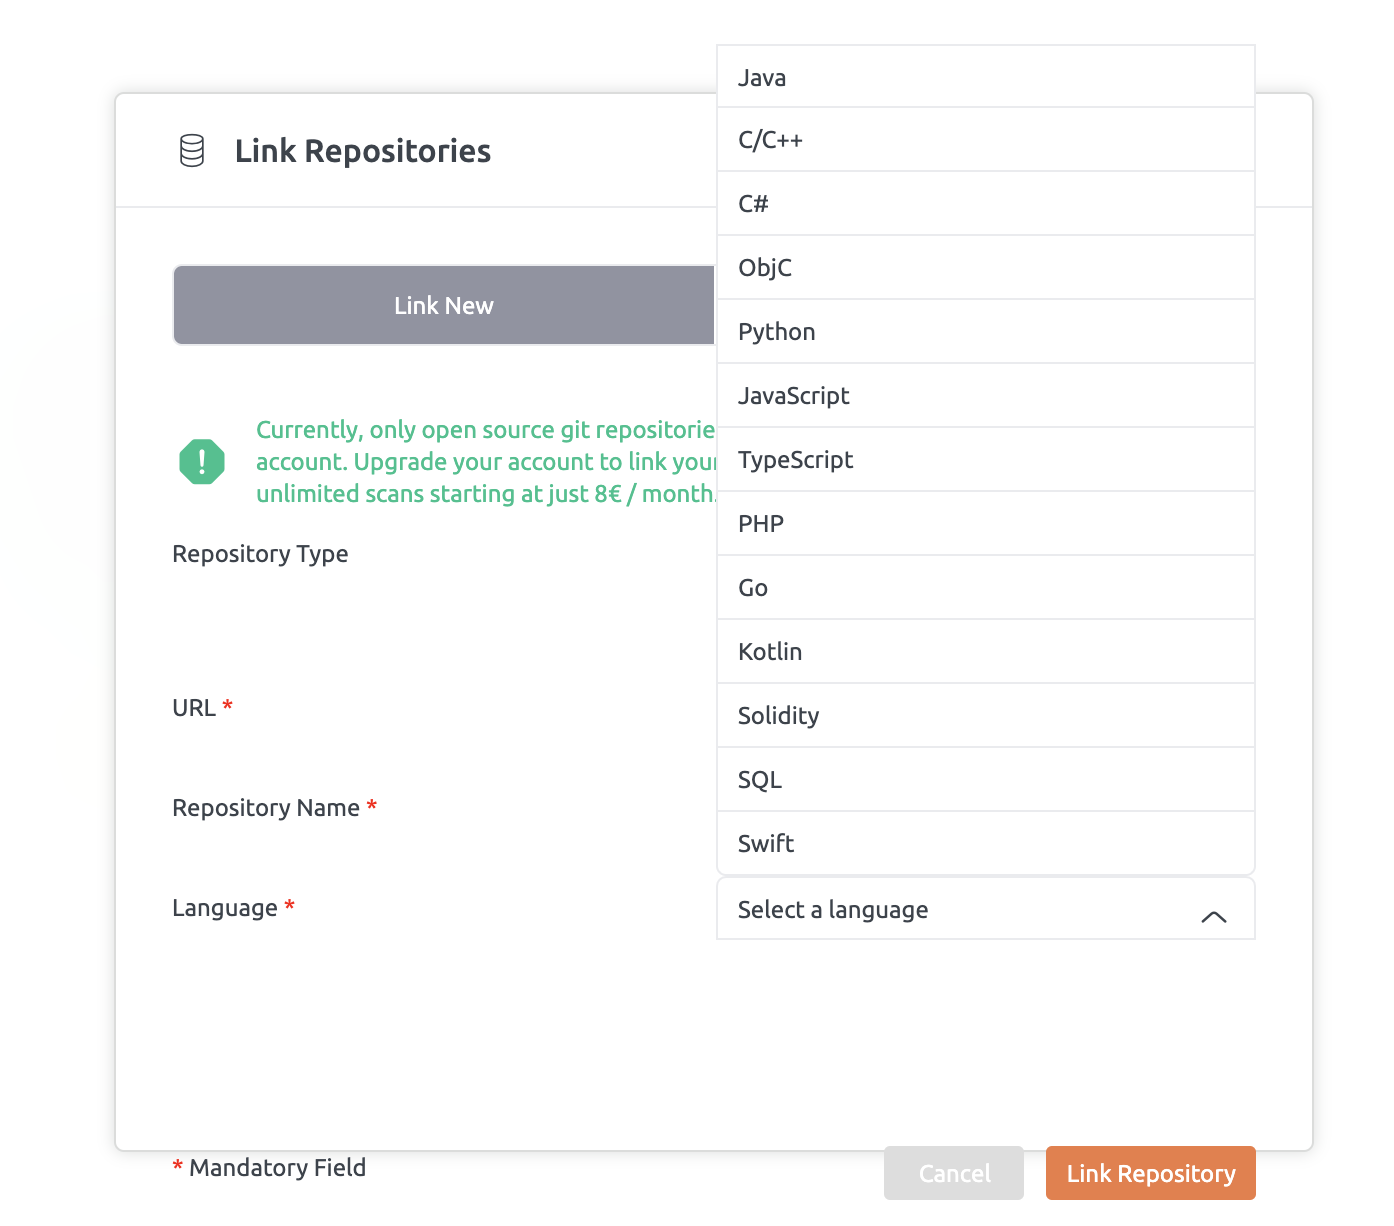
\includegraphics[width=4.5in, height=3in]{negatives.png}
\caption{Programming Languages Availability}
\label{fig:improve}
\end{center}
\end{figure}
\section{Lesson Learned}
I learned about various standards of UX, in depth designing using UCD methodology. It was quite wonderful to have knowledge about the entire design basics and how a little attention could become a big gain for any website. I learnt that it is very important to focus on human needs, extremely important to have iterative approach.\par
It is also important to embrace the change, because human nature is extremely diverse and the most consistent entity in the universe is change. So need to consider ISO standards, work on wireframes and mockups very strongly. Discuss with designers and developers about the design. \par
Along with all this I also got to know about the Embold which is a wonderful tool for various stakeholders in a SDLC. It can be game changer on a healthy scale.






%bibligraphy
\addcontentsline{toc}{chapter}{Bibliography}
\bibliographystyle{plain}
\bibliography{UXbib}



\end{document}